\chapter{Descrição da \textsf{classe-ifg}}
\label{cap:descr}

%% - - - - - - - - - - - - - - - - - - - - - - - - - - - - - - - - - - -
\section{Opções da classe}
\label{sec:opcoes}
Para usar esta classe num documento \LaTeXe, coloque a pasta \verb|formatacao| numa pasta onde o compilador \LaTeX\ pode achá--lo (normalmente na mesma pasta que seu arquivo \verb|.tex|), e defina--o como o estilo do seu documento. Por exemplo, uma dissertação de mestrado:
\begin{verbatim}
\documentclass[dissertacao]{formatacao/classe-ifg}
...
\begin{document}
\end{verbatim}

As opções da classe são \verb|tese| (para tese de doutorado), \verb|dissertacao| (para dissertação de mestrado), \verb|monografia| (para monografia de especialização), \verb|tcc| (para trabalho de conclusão de curso de graduação), \verb|qualificacaom| (para qualificação de mestrado), \verb|qualificacaoe| (para qualificação de especialização), \verb|qualificacaot| (para qualificação de TCC). Se nenhuma opção for declarada, o documento é considerado como uma dissertação de mestrado. Adicionalmente, com a opção \verb|[nocolorlinks]| todos os {\em links} de navegação no texto ficam na cor preta. O ideal é usar esta opção para gerar o arquivo para impressão, pois a qualidade da impressão dos {\em links} fica com qualidade superior. No caso de defesa realizada online inclua a opção \verb|online| para que a folha de aprovação seja gerada sem o espaço para assinatura manual. Caso o curso opte por usar os títulos e cabeçalhos com estilo mais elaborado pode usar também a opção \verb|fancy|.


%% - - - - - - - - - - - - - - - - - - - - - - - - - - - - - - - - - - -
\section{Parâmetros da classe}
\label{sec:param}
Os elementos pré-textuais são definidos página por página e dependem da correta definição dos parâmetros listados a seguir (os elementos que não foram aplicáveis como, por exemplo, \verb|\orientadora| quando orientador é do sexo masculino, devem permanecer comentados usando \% no início da respectiva linha).


Os parâmetros a seguir devem ser preenchidos para todos os tipos de documento:

 \begin{itemize}
\item \verb|\autor| : Nome completo do autor, começando pelo primeiro nome (ex.: \textbf{José da Silva});
\item \verb|\sautor| : Nome completo do segundo autor (quando aplicável), começando pelo primeiro nome (ex.:\textbf{ José da Silva});
\item \verb|\tautor| : Nome completo do terceiro autor (quando aplicável), começando pelo primeiro nome (ex.: \textbf{José da Silva});
\item \verb|\titulo| : Título do trabalho;
\item \verb|\subtitulo| : Se tiver um subtítulo, use este macro para defini-lo;
\item \verb|\tipocurso| : Tipo do curso a que o documento se refere. Coloque uma das seguintes opções: \textbf{Bacharelado}, \textbf{Licenciatura}, \textbf{Especialização}, \textbf{Mestrado Profissional}, \textbf{Mestrado Acadêmico}, \textbf{Doutorado};
\item \verb|\curso| : Nome do curso, excluindo o tipo como, por exemplo, \textbf{Tecnologia de Processos Sustentáveis} ou \textbf{Sistemas de Informação}; 
\item \verb|\campus| : Câmpus (cidade) em que o trabalho foi desenvolvido;
\item \verb|\dia| : Dia do mês da data de defesa (01--31);
\item \verb|\mes| : Mês da data de defesa (01--12);
\item \verb|\ano| : Ano da data de defesa (com quatro dígitos);
\item \verb|\orientador| : Nome completo do orientador, começando pelo primeiro nome;
\item \verb|\unidade| : Unidade do(a) orientador(a) dentro da instituição. No caso de haver mais de um departamento inclua o departamento, a sigla da instituição e o câmpus, como \textbf{Departamento IV - IFG / Câmpus Goiânia}. Em câmpus com um único departamento inclua somente a sigla da instituição e o câmpus, como \textbf{IFG / Câmpus Anápolis}.
\item \verb|\orientadora| : Nome completo da orientadora, começando pelo primeiro nome; use este comando for orientadora e não orientador.
\item \verb|\coorientador| : Nome completo do co-orientador, começando pelo primeiro nome;
\item \verb|\unidadeco| : Unidade do(a) co-orientador(a) dentro da instituição. No caso de haver mais de um departamento inclua o departamento, a sigla da instituição e o câmpus, como \textbf{Departamento IV - IFG / Câmpus Goiânia}. Em câmpus com um único departamento inclua somente a sigla da instituição e o câmpus, como \textbf{IFG / Câmpus Anápolis}.
\item \verb|\coorientadora| : Nome completo da coorientadora, começando pelo primeiro nome; use este comando e o próximo se for coorientadora e não coorientador.
\end{itemize}

Os parâmetros a seguir devem ser preenchidos apenas para dissertações e  qualificações de mestrado:

 \begin{itemize}
\item \verb|\programa| : Programa de Pós-Graduação (ex.: \textbf{Programa de Pós-Graduação Stricto Sensu em Tecnologia de Processos Sustentáveis});
\item \verb|\concentracao| : Área de concentração do programa (ex.: \textbf{Tecnologia de Sistemas de Produção Limpa});
\item \verb|\linha| : Linha de pesquisa do autor (ex.: \textbf{Energias Renováveis e Engenharia Econômica Aplicada}).
\end{itemize}

%% - - - - - - - - - - - - - - - - - - - - - - - - - - - - - - - - - - -
\section{Elementos Pré--Textuais}
\label{sec:pre}
Os elementos pré--textuais são definidos página por página, conforme descritos a seguir:

\paragraph{capa\\}
\verb|\capa| : Gera o modelo da capa externa do trabalho. Nenhum dado é necessário.

\paragraph{rosto\\}
\verb|\rosto| : Gera a folha de rosto, a qual é a primeira folha interna do trabalho. Nenhum dado é necessário.

\paragraph{ficha\\}
\verb|\ficha| : Inclui a ficha catalográfica. Caso seja a defesa final do trabalho inclua a ficha bibliográfico como um arquivo PDF cujo nome deve necessariamente ser \verb|ficha.pdf|. Este arquivo deve estar localizado na mesma pasta que seu arquivo \verb|modelo-ifg.tex|. No caso de exames de qualificação não há necessidade de inclusão da ficha mas \textbf{não altere ou comente o comando}.

\paragraph{termo\\}
\verb|\termo| : Inclui o termo de autorização para disponibilização no repositório digital do IFG. Caso seja a defesa final do trabalho inclua o termo preenchido e assinado como um arquivo PDF cujo nome deve necessariamente ser \verb|termo.pdf|. Este arquivo deve estar localizado na mesma pasta que seu arquivo \verb|modelo-ifg.tex|. O arquivo editável para gerar o termo pode ser obtido em \url{https://www.ifg.edu.br/attachments/article/132/termo\_autorizacao\_rd\_ifg.doc}. No caso de exames de qualificação não há necessidade de inclusão do termo de autorização mas \textbf{não altere ou comente o comando}.

\paragraph{aprovacao\\}
\verb|\aprovacao| : Gera a folha de aprovação para assinatura pelos membros da banca. No caso de exames de qualificação não há necessidade de inclusão da folha de aprovação mas \textbf{não altere ou comente o comando}. No caso de defesa final proceda da seguinte forma: 

\begin{itemize}
\item para gerar o documento antes da defesa preencha o arquivo \verb|pre/preBanca.tex| definindo os membros da banca (com exceção do orientador e do co-orientador). Cada membro deve ser definido usando o comando \verb|\membro| no caso de membro do sexo masculino ou \verb|\membra| no caso de membro do sexo feminino. Deve ser indicado o nome e a unidade do membro como, por exemplo, \verb|\membro{Dr. Fulano de Tal}{Universidade Federal de Goiás (UFG)}|. No caso de defesa online inclua \verb|online| em \verb|\documentclass|.
\item após a defesa e assinatura de todos os membros da banca gere um arquivo PDF cujo nome deve necessariamente ser \verb|aprovacao.pdf| e inclua este arquivo na mesma pasta que seu arquivo \verb|modelo-ifg.tex| e compile novamente o projeto. \textbf{ATENÇÃO:}  caso o arquivo \verb|aprovacao.pdf| seja incluído, a folha de aprovação sem assinaturas não é mais gerada. Dessa forma só inclua esse arquivo na versão final do trabalho.
\end{itemize}

%\paragraph{curriculo\\}
%\verb|\aprovacao| : ambiente para a reprodução do termo de aprovação da Banca Examinadora da tese ou dissertação.
%

\paragraph{dedicatória\\}
\verb|\cdedicatoria| : ambiente para escrever a dedicatória. Usado apenas em defesa final. Inclua o texto da dedicatória editando o arquivo \verb|pre/preDedicatoria.tex|.

\paragraph{agradecimentos\\}
\verb|\cagradecimentos| : ambiente para escrever os agradecimentos. Usado apenas em defesa final. Inclua o texto dos agradecimentos editando o arquivo \verb|pre/preAgradecimentos.tex|.

\paragraph{epígrafe\\}
\verb|\cepigrafe| : macro com 3 argumentos que permite editar um epígrafe. O primeiro argumento é o texto da citação. O segundo argumento é o nome do autor da citação. O terceiro argumento é o ano de nascimento e ano de falecimento (se aplicável) do autor. Usado apenas em defesa final. Inclua os itens da epígrafe editando o arquivo \verb|pre/preEpigrafe.tex|. \textbf{Não remova as chaves (\{ e \}) neste arquivo}.

\paragraph{resumo\\}
\verb|\cresumo| : insere o resumo do trabalho. O texto do resumo deve ser inserido editando o arquivo \verb|pre/preResumo.tex|. A lista das palavras chaves, separadas por `;' deve ser definido antes do ambiente \verb|\resumo|, o qual é usado para escrever o resumo em português.

\paragraph{abstract\\}
\verb|\keys| : insere o abstract do trabalho. O texto do abstract deve ser inserido editando o arquivo \verb|pre/preAbstract.tex|. A lista das palavras chaves em inglês, separadas por `;' deve ser definido antes do ambiente \verb|\abstract|, o qual contém 1 argumento que deve ser o título do trabalho em inglês.

\paragraph{tabelas\\}
\verb|\tabelas| : Macro com 1 argumento opcional para gerar as tabelas. O argumento pode ser:
\begin{itemize}
 \item nada [] : gera apenas o sumário;
 
% fig     -> Gera o sumário e a lista de figuras
% tab     -> Sumário e lista de tabelas
% qua     -> Sumário e lista de quadros
% alg     -> Sumário e lista de algoritmos
% cod     -> Sumário e lista de códigos de programas
% sig     -> Sumário e lista de abreviaturas e siglas
% sim     -> Sumário e lista de símbolos 
 
 \item \textsf{fig} : gera o sumário e uma lista de figuras;
 \item \textsf{tab} : gera o sumário e uma lista de tabelas;
 \item \textsf{qua} : gera o sumário e uma lista de quadros\footnote{A diferença entre tabela e quadro é que tabelas não possuem bordas na lateral ao passo que quadros possuem.};
 \item \textsf{alg} : gera o sumário e uma lista de algoritmos;
 \item \textsf{cod} : gera o sumário e uma lista de programas;
 \item \textsf{sig} : gera o sumário e uma lista de abreviaturas e siglas. Cada sigla deve ser inserida no próprio texto com o comando \verb|\sigla|. Como exemplo, o comando \verb|\sigla{TCC}{Trabalhos de Conclusão de Curso}| gera no texto \textbf{Trabalhos de Conclusão de Curso (TCC)} e insere uma entrada equivalente na lista de abreviaturas e siglas;
 \item \textsf{sim} : gera o sumário e uma lista de símbolos. Diferente de abreviaturas e siglas, os símbolos devem ser inseridos no arquivo \verb|pre/preSimbolos.tex| usando \verb|\simbolo| definindo o símbolo e sua descrição. Na definição do símbolo deve ser usado com formato matemático.
 \item (qualquer outra coisa) : gera somente o sumário.
\end{itemize}

Pode-se usar qualquer combinação dessas opções. Por exemplo:
\begin{itemize}
 \item \textsf{fig,tab} : gera o sumário e listas de figuras e tabelas,
 \item \textsf{fig,tab,cod} : gera o sumário e listas de figuras, tabelas e códigos de programas;
 \item \textsf{fig,tab,alg} : gera o sumário e listas de figuras, tabelas e algoritmos;
 \item \textsf{fig,tab,alg,cod} : gera o sumário e listas de figuras, tabelas, algoritmos e códigos de programas
\end{itemize}

Defina quais listas gerar com base no conteúdo do seu documento.

%% - - - - - - - - - - - - - - - - - - - - - - - - - - - - - - - - - - -
\section{Elementos Textuais}
\label{sec:textuais}

O texto do seu documento deve ser inserido após a definição dos elementos pré-textuais. Para facilitar a organização é recomendado o uso de um arquivo \verb|.tex| para cada capítulo. Os arquivos do texto devem ser inseridos na pasta \verb|tex| e inseridos usando o comando \verb|\input| passando o nome do arquivo como parâmetro (ex. \verb|
\chapter{Introdução}
\label{cap:intro}

Este documento mostra como usar o \LaTeX\ \cite{mittelbach2004latex} com a classe \textsf{classe-ifg} para formatar \sigla{TCC}{Trabalhos de Conclusão de Curso}, monografias, dissertações e teses, assim como exames de qualificação, segundo o padrão adotado pelo Programa de \sigla{PPGTPS}{Pós-Graduação Stricto Sensu em Tecnologia de Processos Sustentáveis} e pela coordenação de Informática do \sigla{IFG}{Instituto Federal de Educação, Ciência e Tecnologia de Goiás} - Câmpus Goiânia. Este documento e a classe \textsf{classe-ifg} foram, em grande parte, adaptados da classe \textsf{inf-ufg} e do texto de \citeonline{infufg} que descreve a sua utilização, ambos vinculados ao Instituto de Informática da Universidade Federal de Goiás. Também foram usadas como referência o Modelo de Teses e Dissertações do \sigla{ICMC}{Instituto de Ciências Matemáticas e de Computação} da \sigla{USP}{Universidade de São Paulo} \cite{icmc-usp} e o Modelo de Teses e Dissertações do \sigla{INPE}{Instituto Nacional de Pesquisas Espaciais} \cite{inpe}.

\LaTeX\ é um sistema de editoração eletrônica muito usado para produzir documentos científicos de alta qualidade tipográfica. O sistema também é útil para produzir todos os tipos de outros documentos, desde simples cartas até livros completos.

Se for necessário algum material de apoio referente ao \LaTeX, consulte o site do \sigla{CTAN}{Comprehensive TEX Archive Network} no endereço \url{http://www.ctan.org/}. Todos os pacotes podem ser obtidos via \siglaestrangeira{FTP}{File Transfer Protocol} \url{ftp://www.ctan.org/} e existem vários servidores em todo o mundo. Eles podem ser encontrados, por exemplo, em \url{ftp://ctan.tug.org/} (EUA), \url{ftp://ftp.dante.de/} (Alemanha), \url{ftp://ftp.tex.ac.uk/} (Reino Unido).

É possível encontrar uma grande quantidade de informações e dicas na página dos usuários brasileiros de \LaTeX\ (\TeX-BR). O endereço é \url{http://biquinho.furg.br/tex-br/}. Tanto no CTAN quanto no \TeX-BR estão disponíveis bons documentos em português sobre o \LaTeX. Em particular no CTAN, está disponível uma introdução bastante completa em português: \url{http://www.ctan.org/tex-archive/info/lshort/portuguese-BR/lshortBR.pdf}. No \TeX-BR também existe um documento com exemplos de uso de \LaTeX\ e de vários pacotes: \url{http://biquinho.furg.br/tex-br/doc/LaTeX-demo/}. O objetivo é ser, através de exemplos, um guia para o usuário de \LaTeX\ iniciante e intermediário, podendo, ainda, servir como um guia de referência rápida para usuários avançados.

Se desejar usar o \LaTeX\ instalado no computador, verifique em quais sistemas ele está disponível em \url{http://www.ctan.org/tex-archive/systems/}. Em particular para \textsf{MS Windows}, o sistema gratuito \href{http://www.miktex.org/}{MikTeX}, disponível no CTAN e no site \url{http://www.miktex.org/} é completo e atualizado.

O estilo \textsf{classe-ifg} se integra completamente ao \LaTeXe. Uma dissertação ou monografia escrita no estilo padrão do \LaTeX\ para teses (estilo \verb|report|) pode ser formatada em 15 minutos para se adaptar às normas do IFG.

O estilo \textsf{classe-ifg} foi desenhado para minimizar a quantidade de texto e de comandos necessários para escrever seu documento. Só é preciso inserir algumas macros no início do seu arquivo \LaTeX, precisando os dados bibliográficos da sua dissertação (por exemplo o seu nome, o titulo da dissertação\ldots). Em seguida, cada página dos elementos pré-textuais será formatada usando macros ou ambientes específicos. O corpo do texto é editado normalmente. Finalmente, as referências bibliográficas podem ser entradas manualmente (via o comando \verb|\bibitem| do \LaTeX\ padrão) ou usando o sistema BiBTeX (muito mais recomendável). Neste caso, os arquivos \verb|abnt-alf.bst| e \verb|abnt-num.bst| permitem a formatação das referências bibliográficas segundo as normas da \citeonline{abnt}.

|) onde \verb|cap01| é o arquivo definido.

É a ordem de inclusão dos arquivos e não seu nome que define o capítulo que será gerado. Dessa forma, os comandos abaixo

\begin{Verbatim}
\input{./tex/arquivox}
\input{./tex/arquivoy}
\end{Verbatim}

farão com que o conteúdo do arquivo \verb|arquivox.tex| gerem o Capítulo 1 do documento e que o conteúdo do arquivo \verb|arquivoy.tex| gerem o Capítulo 2. 

Caso deseje remover um capítulo basta comentar ou remover o comando \verb|input| equivalente.

%% - - - - - - - - - - - - - - - - - - - - - - - - - - - - - - - - - - -
\section{Bibliografia}
\label{sec:bib}

A bibliografia é inserida através do comando \verb|\bibliografia|. Os documentos citados devem ser inseridos editando o arquivo \verb|bib/bibliografia.bib| usando o formato \BibTeX, uma ferramenta de formatação usada em documentos \LaTeX. O Anexo \ref{anexo:referencias} fornece uma lista de tipos de referência usando esta ferramenta. 

Geralmente a página da publicação disponibiliza o formato \verb|.bib|. Outra maneira de obter esta entrada é defini-la manualmente ou realizar a busca na ferramenta \href{https://scholar.google.com}{Google Scholar} clicando nos links \textbf{Cite} (Figura \ref{fig:scholar01}) e \textbf{BibTeX} (Figura \ref{fig:scholar02}). 

\begin{figure}[H]
  \centering
  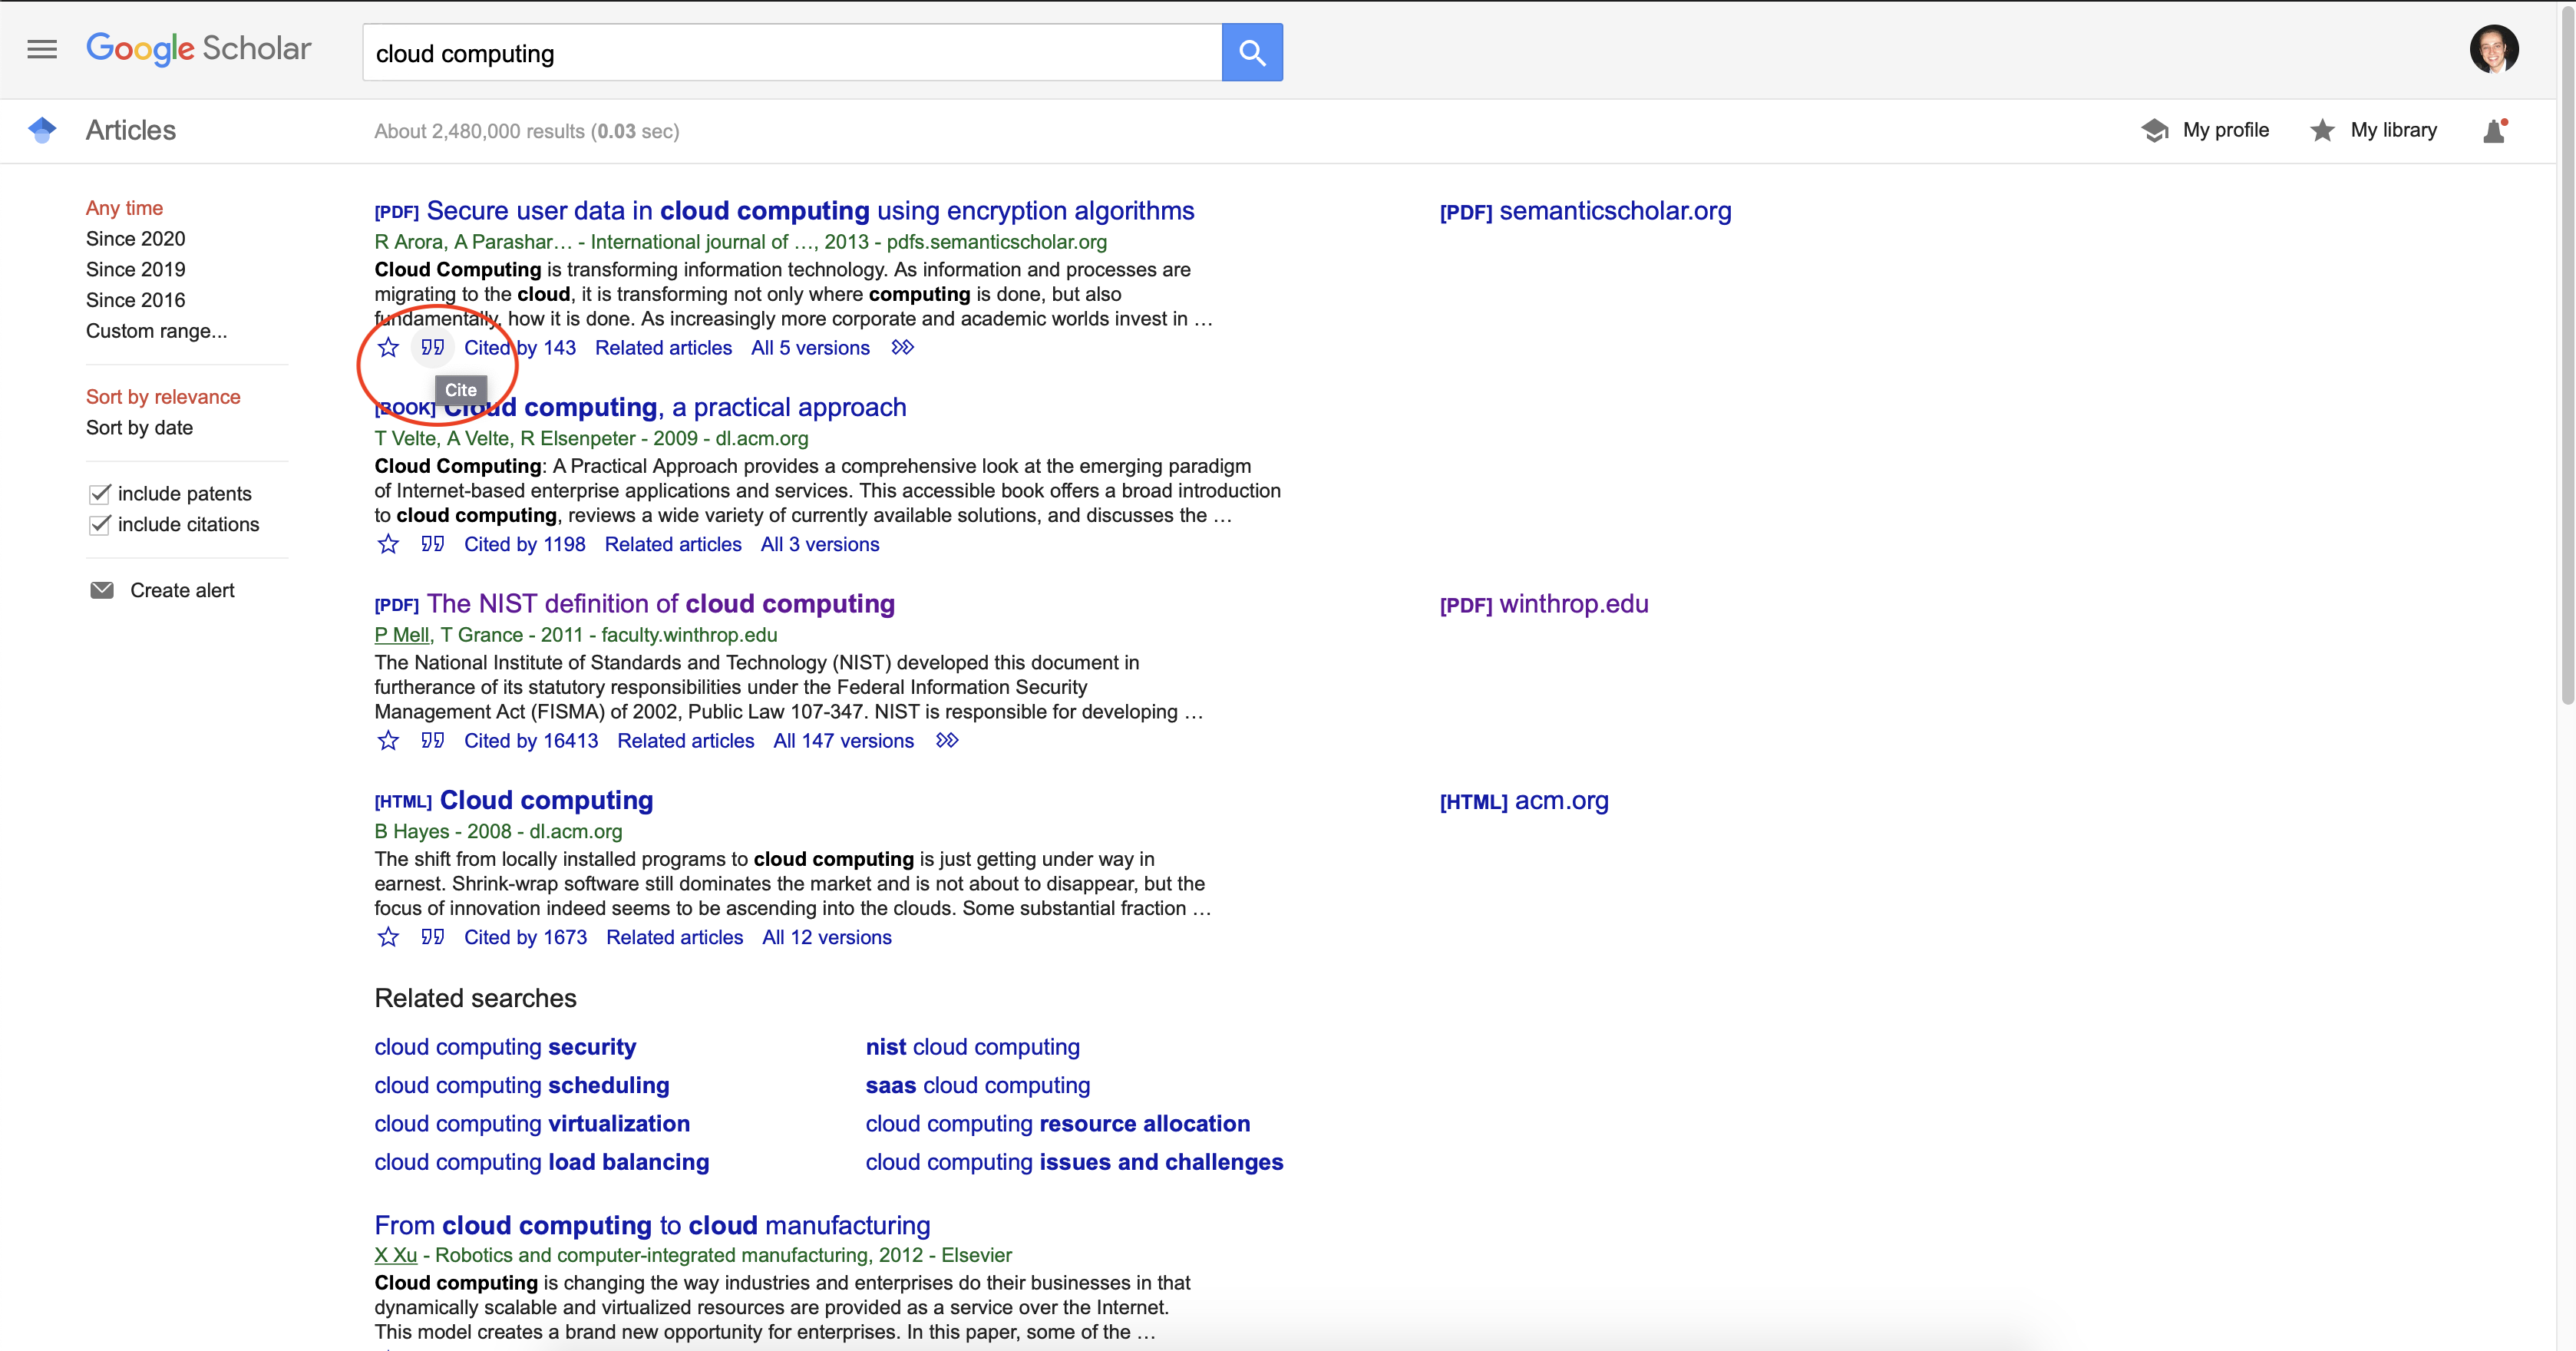
\includegraphics[width=1.0\textwidth]{./fig/scholar01}
  \caption{Busca de referência no formato .bib usando Google Scholar - Primeira tela.}
  \label{fig:scholar01}
  \fontefig{Elaborado pelo autor}
\end{figure}

\begin{figure}[H]
  \centering
  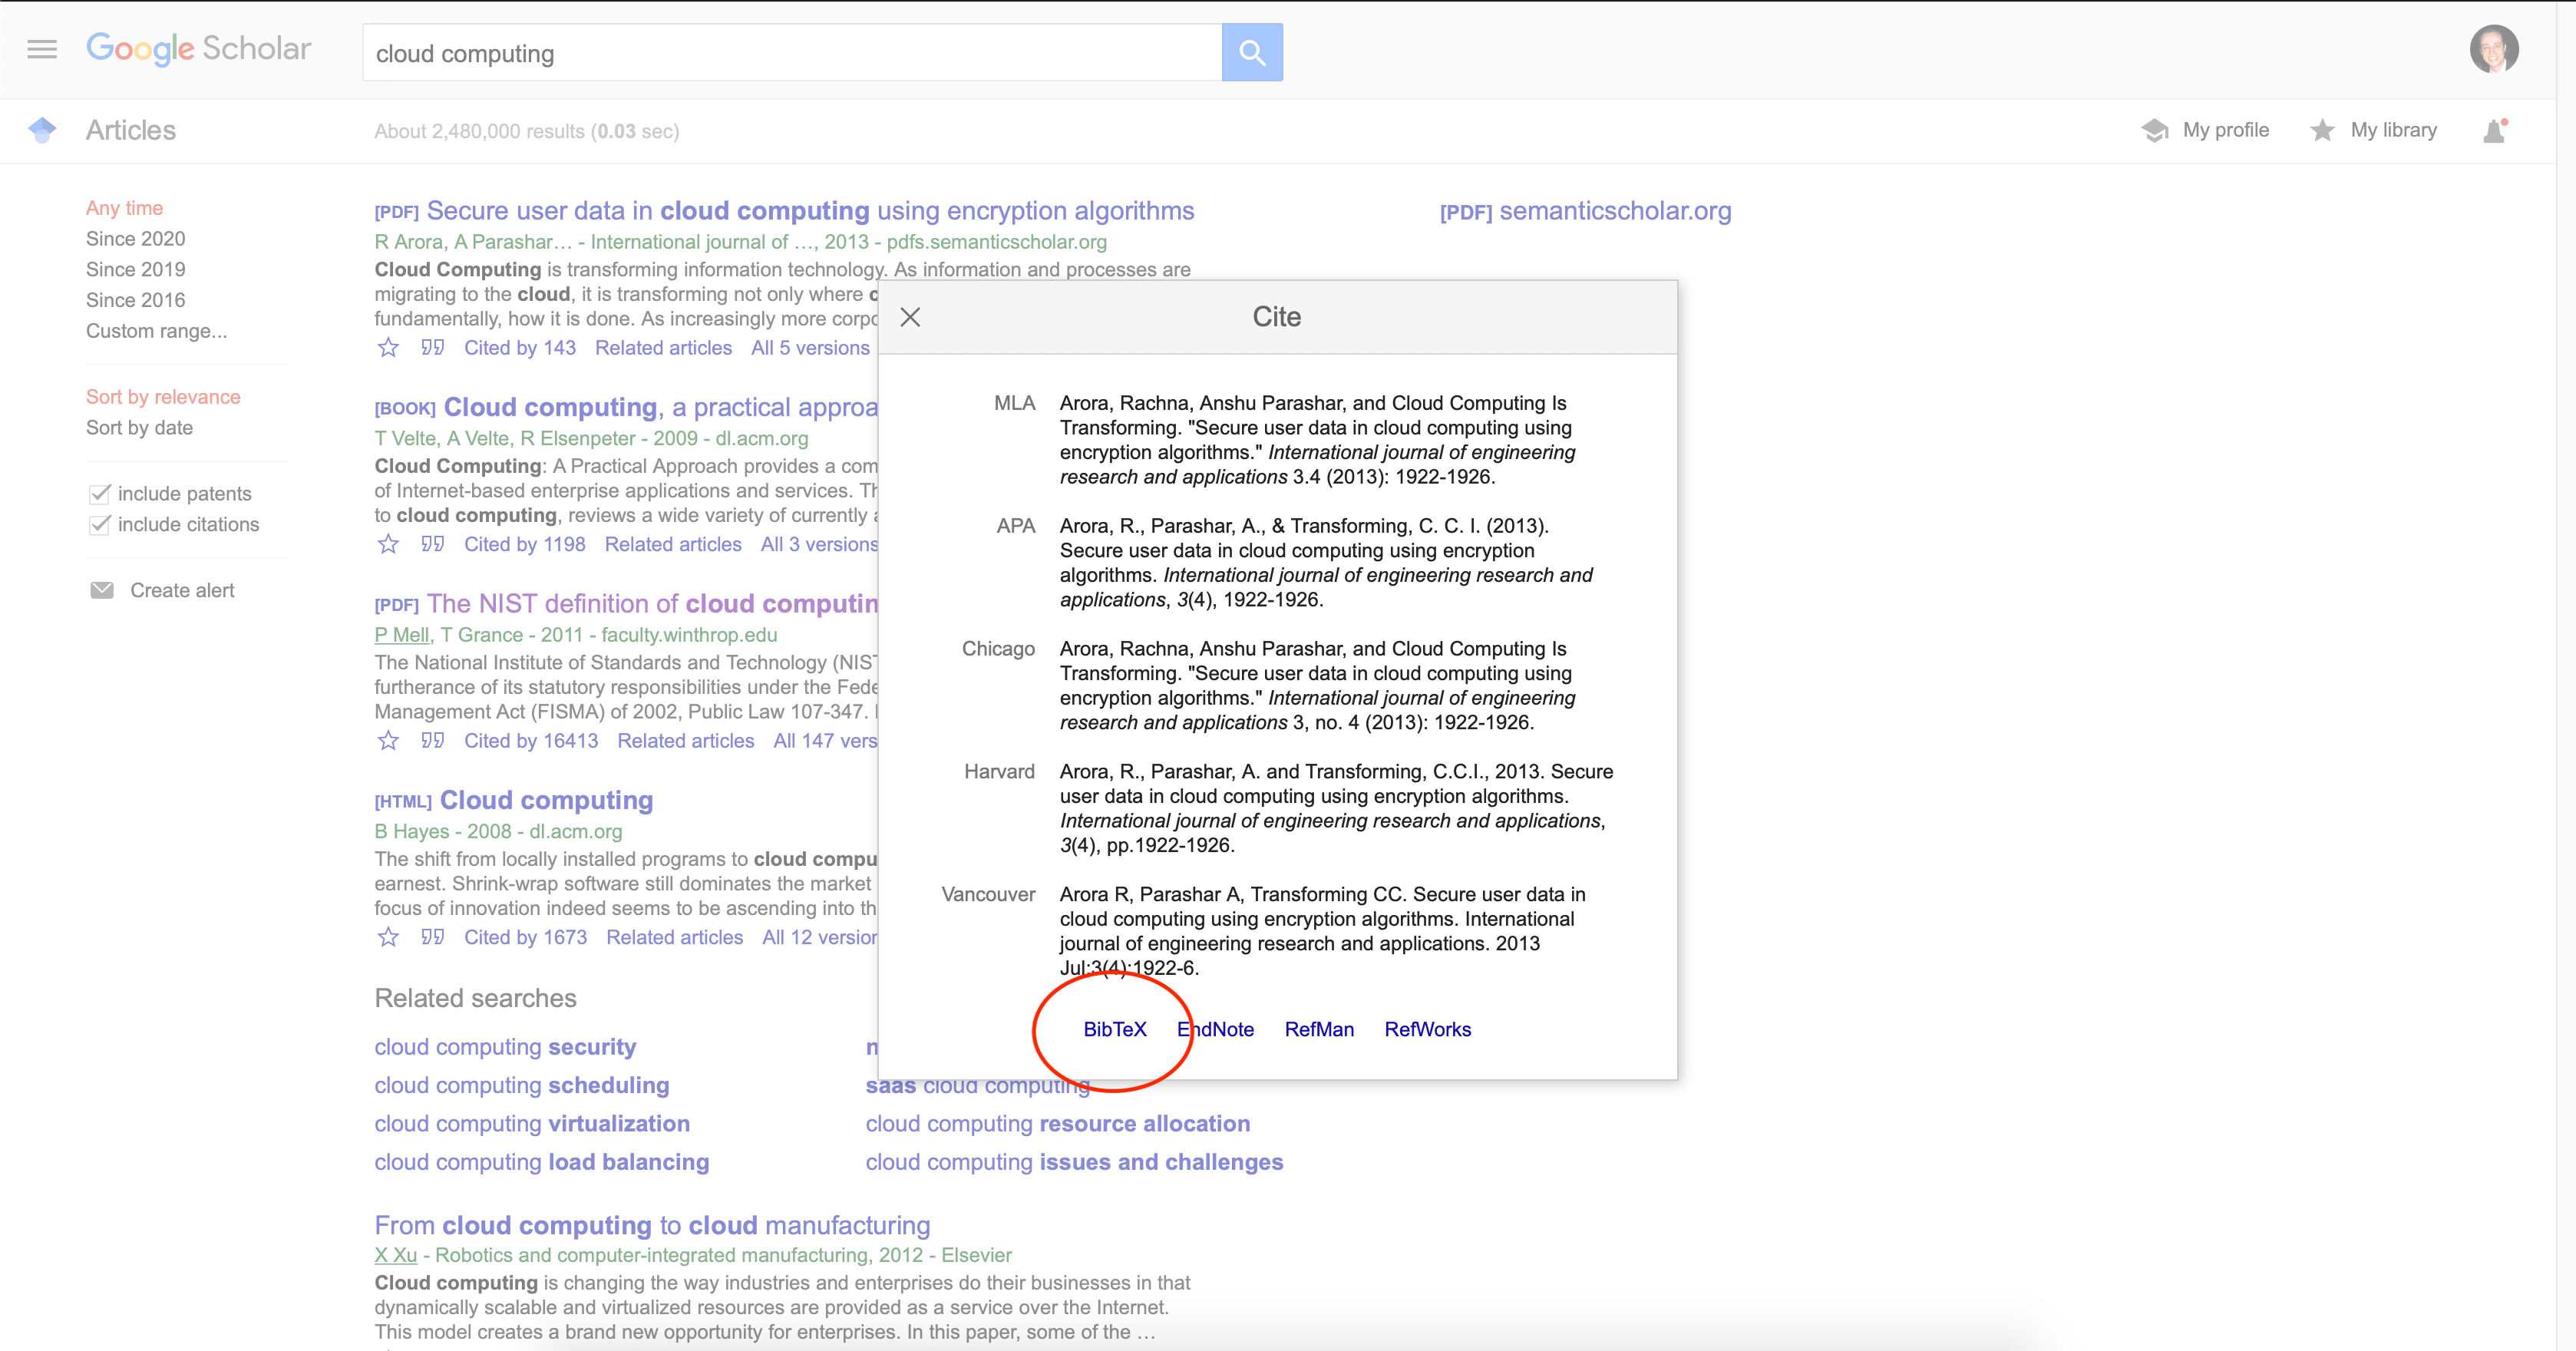
\includegraphics[width=1.0\textwidth]{./fig/scholar02}
  \caption{Busca de referência no formato .bib usando Google Scholar - Primeira tela.}
  \label{fig:scholar02}
  \fontefig{Elaborado pelo autor}
\end{figure}

Apenas referências citadas no texto aparecem no documento gerado. Dessa forma, não é necessário se preocupar em remover do arquivo \verb|bibliografia.bib| aquelas que não serão mais utilizadas.

\section{Elementos Pós--Textuais}
\label{sec:pos}

Os elementos pós-textuais constituem apêndices e anexos. A principal diferença entre anexo e apêndice é que os apêndices são textos criados pelo próprio autor para complementar sua argumentação, enquanto os anexos são documentos criados por terceiros, e usados pelo autor. 

A inserção de apêndices deve ser realizada após o comando \verb|\apendices|, da mesma forma que a inclusão de capítulos (um arquivo para cada apêndice). A única diferença é que os arquivos devem ser inseridos na pasta \verb|apendices|. Do mesmo modo, os anexos devem ser inseridos após o comando \verb|\anexos|, com os arquivos colocados na pasta \verb|anexos|.